\section{Lateral weirs in HECRAS and \anuga{}}

This test compares riverwalls in ANGUA with default lateral structures in
HECRAS. 

\begin{figure}
\begin{center}
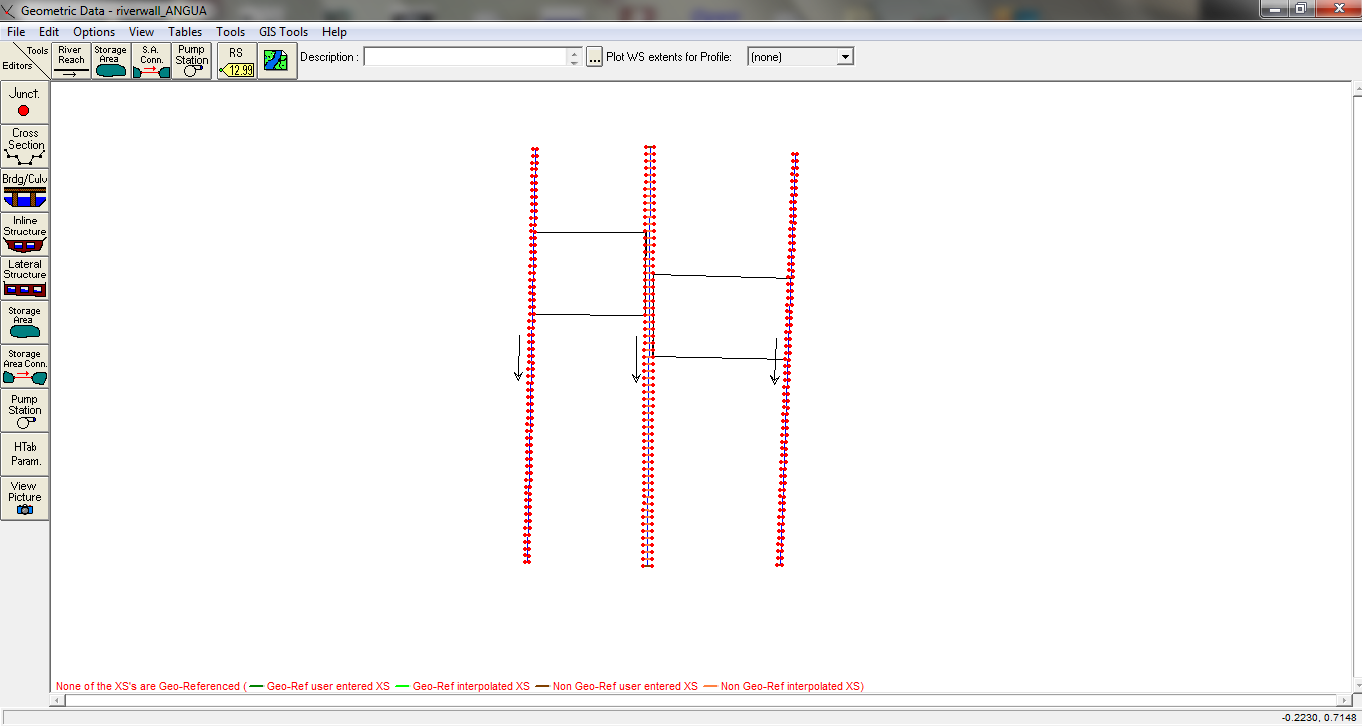
\includegraphics[width=0.9\textwidth]{hecras_riverwall_anugaTest/RASGeometry_levee.png}
\end{center}
\caption{HECRAS model geometric schematization. The `right' channel appears on
the left side of this figure, and the `left' on the right.}
\label{schematic}
\end{figure}

A HECRAS model was set up with 3 uniform parallel channels (`left', `middle',
`right', orientations defined when looking downstream). All channels had
lengths of 1000m, bed-slope $3/1000$, manning's n of 0.03, while their widths were 10m,
20m, and 10m respectively (Figure~\ref{schematic}). The cross-sections were all
nearly-flat (three-points with bank elevations 1cm above the central bed
elevation), and for all reaches the most upstream cross-section (1000) had an
elevation of 0m. These three channels were connected with broad-crested lateral
weirs (using HECRAS's default lateral weir drag coefficient of 1.1 in metric
units). The `right' and `middle' channels were connected with a 198m long weir
with an elevation 0.5m above the bed, from stations 799 to 601. The `left' and
'middle' channels were connected with a 198m long weir with an elevation 0.5m
above the bed from stations 699 to 501. 

Throughout the simulation the `left' and `right' channels were given a
discharge of 0.1m$^3$/s (just enough to prevent them drying, which causes numerical
blow-up in in HECRAS). The `middle' channel was given a discharge timeseries,
increasing from 1m$^3$/s to 21m$^3$/s over a few hours of simulated time. The entire model
is run for 24hours.

As the discharge in the central channel increases, water starts to overtop the
riverwalls and flows into the side channels. The loss/gain and final
equilibrium flow state in each channel is determined by the flow over the
riverwalls, which is itself a function of the stage in each river. Although
both riverwalls are 0.5m above the bed, the `right' channel receives more water
than the `left' channel because it has the most upstream connection to the
`middle' channel. Further downstream the `middle' channel has already lost a
significant part of its discharge, so it flows less deeply and there is less flux over
the more downstream riverwall.

An analogous ANUGA model was set up with riverwalls connecting 3 channels. The
`Qfactor' for both riverwalls was set to (1.1/1.7$\simeq$0.65) to make the
ANUGA riverwall drag coefficient equivalent to the default HECRAS drag
coefficient (the default Qfactor in ANUGA is 1). The same discharge timeseries
and elevations were used. The manning's n values were slightly increased to
account for the fact that HECRAS uses side-wall friction in the channels,
whereas ANUGA doesn't. The correction was derived by equating the ANUGA and
HECRAS friction slope terms assuming a final flow depth of $d \simeq 0.5m$, and
channel width of $ w \simeq 10$m. Denoting $n_{A}$ as ANUGA's manning's n and
$n_{H}$ as HECRAS's value (0.03), we have:
\begin{equation}
n_{A} \simeq n_{H}\frac{d^{2/3}}{( \frac{dw}{2d + w} )^{2/3}} \simeq 0.032
\end{equation}
where the denominator on the right hand side is the hydraulic radius. This
correction is not exact since the depths and widths actually vary, but despite
those second order effects it does improve the agreement between the 2 models.

The initial conditions in each model are slightly different but this is only
important in the first hour of simulation. HECRAS needs 'well-behaved' initial
conditions to maintain stability. 

\subsection{Results}

Figures~\ref{midReach}-\ref{leftReach} show stage timeseries at various
stations downstream in each channel. The results are qualitatively similar,
with stages typically differing by a few cm. In the downstream parts of the
left/right channels, the stage is completely determined by the mass flux over
the upstream weirs, and so the agreement between HECRAS and ANUGA here shows
that both models are predicting a similar mass flux.

The main difference between the 2 models is in areas just upstream of the weir
(800 on the right channel, 700 on the left), where HECRAS predicts a greater a
backwater effect in the receiving channel than ANUGA. Further investigation has
shown this is because of differences in the transport of momentum over the
riverwall. HECRAS apparently only transfers mass over the weir, whereas ANUGA
transfers both mass and momentum. This causes more stagnation at the upstream
parts of the riverwall overflow in HECRAS, since the water is transferred to
the side channels without a downstream component of momentum. We have done
other ANUGA runs where the momentum flux over the weir was forced to zero (by
modifying ANUGA's source code), and in that instance the models agree well in
the aforementioned areas as well.

Irrespective, the main point of this comparison is that both ANUGA and HECRAS
are giving similar results for this case study. 


\begin{figure}
\begin{center}
\includegraphics[width=0.9\textwidth]{MIDDLE_REACH.png}
\end{center}
\caption{Stage at various points downstream in the middle channel}
\label{midReach}
\end{figure}

\begin{figure}
\begin{center}
\includegraphics[width=0.9\textwidth]{RIGHT_REACH.png}
\end{center}
\caption{Stage at various points downstream in the right channel}
\end{figure}

\begin{figure}
\begin{center}
\includegraphics[width=0.9\textwidth]{LEFT_REACH.png}
\end{center}
\caption{Stage at various points downstream in the left channel}
\label{leftReach}
\end{figure}


\endinput
